\section{Experiment}
%We designed and implemented a series of experiments to evaluate the
%performance of our approach.
This section describes the experiment settings and analyses the
experiment results.
Experiments described in this section mainly made use of the following
data:
\begin{itemize}
\item \textbf{Keyword set:} a massive dataset consisting of 0.702
billion bid phrases.
\item \textbf{Query set:} a collection of 30 million search queries.
\item \textbf{Search logs:} 15.5 billions of records of the
form: <query:str, bid phrase:str, $\ldots$, click-or-not:bool> within
which there exist 0.83 billion distinct queries.
\end{itemize}
All these data are provided by a commercial search engine and the
search log is accumulated during one month period of time.
%We firstly checked the effectiveness of proposed disambiguation
%approach.
%After conceptualization, bid phrases are mapped into our concept space.
%To expand a query, we firstly select candidate bid phrases for it.
%So experiment is made to comparison between our candidates
%selection approaches (i.e., CSCD and CSJS).
%%We estimate the similarity between each candidate with a given query by
%%SMS.
%Then candidates are ranked based on SMS.
%Thus, we evaluated SMS before assessing the resulting suggestions
%(expansions) of a given query.
%%In our third experiment, we observed a
%%strong positvie correlation between SMS and search users' interests.
%Finally, to show that proposed approach is effective for query
%expansion and keyword suggestion, we assessed the relevance between
%retrieved bid phrases and the given queries.
    %We designed and implemented the following experiments to examine the
%performance of our approach:
%\begin{enumerate}
%\item We begin evaluating our approach with semantic-matching score(SMS).
%%We assign SMS to each candidate bid phrase based on similarity between
%it and given query.
%\item we evaluate the quality of retrieved bid phrases.
%%In contrast to traditional IR which only focuses on the relevance
%%between retrieved documents and given query, we prefer to bid phrases
%%which are not obvious yet relevant.
%\item We make comparison between candidates selection approaches
%proposed in this paper.
%\end{enumerate}
%To prove the efficacy of semantic-matching score proposed in our
%approach, we mined click-through data to evaluate the correlationship
%between CTR and computed semantic-matching score.
%We sampled several queries from search log and generated expansion for
%them using both traditional term matching scheme and our approach.
%User study was held to compare the quality of resulting expansions.
%We also compared the performance of different candidates selection
%approaches proposed in this paper on specific domain.
%Finally, we report the result of flight analysis supported by Bing
%search engine.
%It not only reveals the scalability and efficiency of our approach,
%   but also a more credible evaluation for effectiveness.
\subsection{Disambiguation}
With rich isA relationships, knowledge-based approaches can map
terms to their synonyms and similar varieties through their hypernyms.
However, existing approaches neglected polysemy which is also
prevalent especially within bid phrases. We have emphasized that
leveraging our co-occurrence network, we can identify the appropriate
sense of detected instnace, so we made experiment to evaluate the
effect of our disambiguation approach.


We randomly sampled one million bid phrases from our keyword set and
then extracted those containing ambiguous instances ``apple'',
     ``blackberry'', ``palm'', ``bass'' and ``mouse'' as our test set.
We applied our approach to conceptualize each of these bid phrases.
Thus each occurrence of the five ambiguous instances is explicitely
associated with one of its sense.
Regarding the disambiguation as a classification problem, we manually
labeled correct sense for these ambiguous instances appeared in test
set and adopted accuracy as metrics to access the effect of our
disambiguation approach.


The experiment results are presented in Table \ref{tab:acc}. The
classification accuracy of ``bass'' seems not satisfiable because
multi-class classification is much more tough in most cases. Most of
the miss classified samples of ``apple'' are those which refer to
``tree'' but associated with ``fruit'' and vice versa. The reason is
that seperating these two senses from ``company'' is easy but the two
senses themselves are somehow similar. It is more difficult to
identify the proper sense under a smaller granularity.
\begin{table}
\centering
\begin{tabular}{|c|c|c|c|c|}\hline
instance&\#senses&\#correct&\#sample&accuracy\\\hline
apple&3&157&171&0.918\\\hline
blackberry&2&127&142&0.894\\\hline
palm&3&76&84&0.905\\\hline
bass&4&46&57&0.807\\\hline
mouse&2&184&200&0.920\\\hline
\end{tabular}
\caption{Accuracy of disambiguation}
\label{tab:acc}
\end{table}
\subsection{CSCD v.s. CSJS}
%\subsection{Candidates Selection Comparison}
\textbf{Objective} of this experiment is to compare the two candidates
selection approaches proposed in this paper.
%Although Probase is full of common sense knowledge which can be used
%for general purpose task and approach proposed in our paper is
%intended to resolve open-domain keyword suggestion and query expansion.
The CSCD (see Subsection \ref{sec:CSCD}) mines click-through data to
extract co-click relationships between queries.
Although the co-click relationships capture semantic relatedness
between queries accurately, there are inadequate click-through data for
tail queries.
Thus, CSCD can't be applied for tail queries.
On the other hand, CSJS (see Subsection \ref{sec:CSJS}) directly
leverages semantic knowledge provided by Probase and thus has broader
application scenarios than CSCD.


\textbf{Dataset} used for this experiment includes our keyword set as
well as 21 queries randomly sampled from our search logs.
These queries are all related to a specific domain---``hotel''.
%Thus, we compare the two different candidates selection
%approaches---CSCD and CSJS(see subsection \ref{sec:CSJS}) using queries all belong to a very popular
%topic---``hotel''.
%It is still meaningful for us to evaluate the performance of our
%approach for queries of a specific domain especially popular
%topics(e.g., travel, hotel, insurance, etc.) because search engines
%usually provide vertical search engines for them which are designed
%for a certain specific domain and usually achieve better
%performance on their corresponding domain compared with general
%purpose approach.
%We randomly sampled 21 queries from search log which are all related
%to ``hotel'' topic.
Because ``hotel'' is one of the three most popular topics(i.e.,
        ``travel'', ``hotel'', ``insurance'') of sponsored search,
        there is sufficient click information for these sampled
        queries, and thus CSCD can perform well for them.


For each sampled query, we ranked candidate bid phrases that are
selected by CSCD and CSJS respectively based on SMS and reserved at
most top-$30$ as retrieval results.
%We select relevant bid phrases for sampled queries from 702 millions
%of bid phrases contained by a commercial search engine using framework
%proposed in this paper while different candidates selection approaches.



\textbf{Metrics} used for accessing retrieved results %of the two
%approaches
is average precision at N (\emph{P@n})
    \cite{baeza2011modern}.
We manually labeled more than 1200 query-bid phrase pairs
according to the labeling guideline listed in Table
\ref{tab:scoringrule}.
We computed P@n by regarding bid phrases with score 1 or 2 as
good(positive) cases, and average \emph{``extreme''} precision at n by
regarding only bid phrases with score 2 as good(positive) cases.
\begin{table}
\centering
\begin{tabular}{|c|c|}\hline
Score (Label)&Reasons\\\hline
2 point      &Synonymy;Word Permutation;\\
very relevant&CAL;Disambiguation.\\\hline
1 point&Subset;Overlap;\\
somewhat relevant&Superset;Similar.\\\hline
0 point   &Clarion hotels$\rightarrow$\\
Irrelevant&hotels rewards cards\\
\hline
\end{tabular}
\caption{Labeling Guideline for Hotel Queries and Bid Keywords}
\label{tab:scoringrule}
\end{table}
%We also compare different candidates selection approaches.
%Selection by measuring Jaccard Similarity and Overlap Similarity is
%denoted as Approach\uppercase\expandafter{\romannumeral1} while
%selection by exploiting co-click information is denoted as Approach\uppercase\expandafter{\romannumeral2}.
\begin{table}[!ht]
\centering
\begin{tabular}{|p{2cm}|c|c|c|c|}
\hline
label&\multicolumn{2}{|c|}{CSJS}&\multicolumn{2}{|c|}{CSCD}\\
\cline{2-5}
     &\#count&ratio&\#count&ratio\\
\hline
0&15&0.062&2&0.010\\
\hline
1&174&0.719&90&0.429\\
\hline
2&53&0.219&118&0.562\\
\hline
P@10&\multicolumn{2}{|c|}{93.80\%}&\multicolumn{2}{|c|}{99.05\%}\\
\hline
extreme P@10&\multicolumn{2}{|c|}{21.90\%}&\multicolumn{2}{|c|}{56.19\%}\\
\hline
\end{tabular}
\caption{P@10 of CSJS and CSCD}
\label{tab:pat10}
\end{table}
\begin{table}[!h]
\centering
\begin{tabular}{|p{2cm}|c|c|c|c|}
\hline
label&\multicolumn{2}{|c|}{CSJS}&\multicolumn{2}{|c|}{CSCD}\\
\cline{2-5}
     &\#count&ratio&\#count&ratio\\
\hline
0&38&0.082&3&0.007\\
\hline
1&332&0.719&196&0.467\\
\hline
2&92&0.199&221&0.526\\
\hline
P@20&\multicolumn{2}{|c|}{91.77\%}&\multicolumn{2}{|c|}{99.29\%}\\
\hline
extreme P@20&\multicolumn{2}{|c|}{19.91\%}&\multicolumn{2}{|c|}{56.62\%}\\
\hline
\end{tabular}
\caption{P@20 of CSJS and CSCD}
\label{tab:pat20}
\end{table}



\textbf{Experiment results} are illustrated in Table \ref{tab:pat10} and
Table \ref{tab:pat20}.
%Approach\uppercase\expandafter{\romannumeral1}
As you can see, CSCD outperforms CSJS which confirms the intuition that
co-click relationships can accurately capture semantic relatedness.
%\uppercase\expandafter{\romannumeral2}.
%It benefits from click-through data which provide useful hints for
%selecting highly relevant bid phrases as candidates.
However, not all topics are as popular as ``hotel''.
%In many cases, queries related to rare topics are seldom accessed
%by search users.
When there is no sufficient click-through data for CSCD to draw
reliable conclusions, CSJS will function as CSCD's complement.
\subsection{Validating Semantic-Matching Score}
%Ranking function assigns scores to documents with regard to a given query~\cite{baeza2011modern}.
%Our approach is of no exception.
%We assigned \emph{SMS} to each bid phrase with respect to a given
%query.
We ranked candidate bid phrases by \emph{SMS} and select the
top-ranking ones as resulting expansions for the issued query.
Obviously, only when SMS reflects the relevance between short texts
accurately can we rank bid phrases in a reasonable order.
\subsubsection{Ground Truth}
As we know, click thorugh rate (\emph{CTR}) of an ad is defined as the
number of clicks on this ad divided by the number of the ad's
impressions.
High CTR indicates successful advertising campaign.
Because the matching of query to ads is through bid phrases, we can
apply CTR for bid phrases by simply accumulating impressions according
to bid phrases instead of ads.
Accordingly, we define CTR of query-bid phrase pair as follow:
\begin{definition}
\label{def:ctr}
Given query $q$ and bid phrase $p$, we have
\begin{equation}
\text{CTR}(q,p)=\frac{\text{Clicks}(q,p)}{\text{Impressions}(q,p)}\times
100\%
\end{equation}
where both clicks and impressions are triggered by bid phrase $p$ in
response to query $q$.
\end{definition}
We extracted tuples in the form $<query:string, bid
    phrase:string, click-or-not:bool>$ from our search logs.
Then we computed CTR of each query-bid phrase pair by aggregating all
these tuples over their first two columns.



%Then we can use CTR of query-bid keyword pair as the actual similarity
%or at least a high-quality approximation of similarity between the
%query and bid keyword.
%So we can check that whether semantic-matching score makes sense in
%terms of representing the similarity between short text by analysing
%the correlation between CTR and it.
We made assumption that CTR of query-bid phrse pair is proportional to
their semantic similarity and used CTR as ground truth.
Thus, to check whether SMS properly reveals semantic similarity between short
texts, we check whether there exists a strong positive correlation
between SMS and CTR.
In another word, if higher SMS corresponds to higher CTR and lower SMS
corresponds to lower CTR, we have confidence to announce that SMS can
reflect semantic similarity between short texts accurately.
\subsubsection{SMS v.s. CTR}
We quantitate SMS evenly into ten intervals denoted by integral
identifiers ranging from 1 to 10 where interval with larger identifier
corresponds to higher SMS.
To observe the relationship between SMS and CTR, we present Figure
\ref{fig*:subfig:a}.
Horizontal axis of it represents the identifiers of SMS intervals.
%semantic-matching score of query-bid keyword pair. We quantitate it
%into ten buckets denoted by integers from 1 to 10 where larger integer
%means higher semantic-matching score.
Vertical axis of it represents the average CTR of query-bid phrase
pairs.
As you can see, pairs with higher SMS have higher CTR.
There exists a strong positive correlation between them which persuasively
proves the effectiveness of SMS.
%Although the number of impressions does not increase monotonically.
%It overall also reveals strong correlation with semantic-matching
%score.
\begin{figure*}[!t]
    \subfigure[Different SMS Range] {
        \label{fig*:subfig:a}
        \begin{minipage}[b]{0.33\textwidth}
            \centering
            %\epsfig{file=figures/correlation.eps,height=1.2in,width=2.2in}
            \includegraphics[height=1.2in,
                width=2.2in]{figures/correlation.eps}
        \end{minipage}}%\vspace{-1.0mm}
    \subfigure[Head Queries] {
            \label{fig*:subfig:b}
            \begin{minipage}[b]{0.33\textwidth}
            \centering
            %\epsfig{file=figures/headdecile.eps,height=1.2in,width=2.2in}
            \includegraphics[height=1.2in,
                width=2.2in]{figures/headdecile.eps}
        \end{minipage}}%\vspace{-1.0mm}
    \subfigure[Torso Queries] {
            \label{fig*:subfig:c}
            \begin{minipage}[b]{0.33\textwidth}
            %\epsfig{file=figures/torsodecile.eps,height=1.2in,width=2.2in}
            \includegraphics[height=1.2in,
                width=2.2in]{figures/torsodecile.eps}
        \end{minipage}}\\
    \subfigure[Tail Queries] {
        \label{fig*:subfig:d}
        \begin{minipage}[b]{0.33\textwidth}
        \centering
            %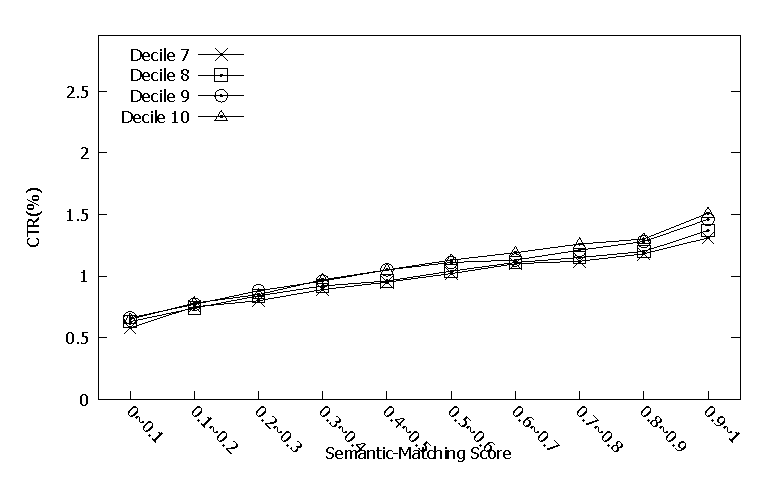
\epsfig{file=figures/taildecile.eps,height=1.2in,width=2.2in}
            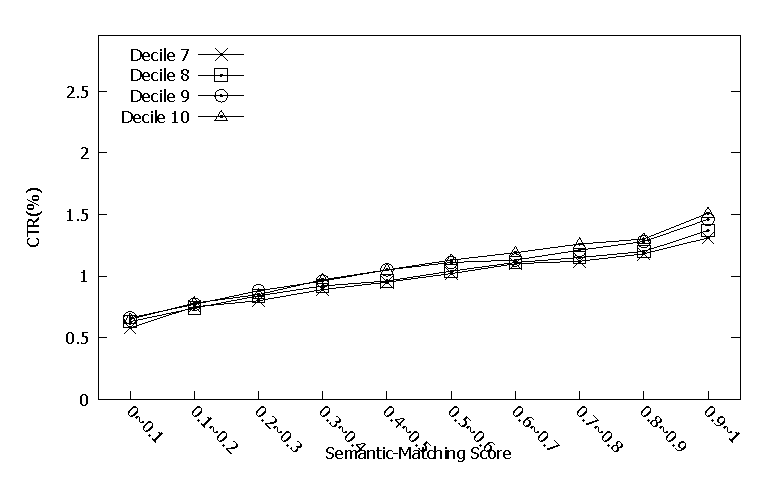
\includegraphics[height=1.2in,
                width=2.2in]{figures/taildecile.eps}
        \end{minipage}}%\vspace{-1.0mm}
    \subfigure[Mainline Ads] {
        \label{fig*:subfig:e}
        \begin{minipage}[b]{0.33\textwidth}
        \centering
            %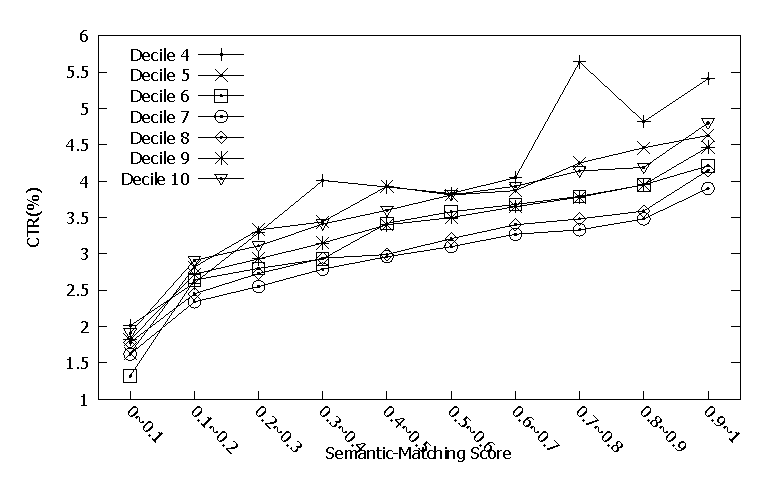
\epsfig{file=figures/ml.eps,height=1.2in,width=2.2in}
            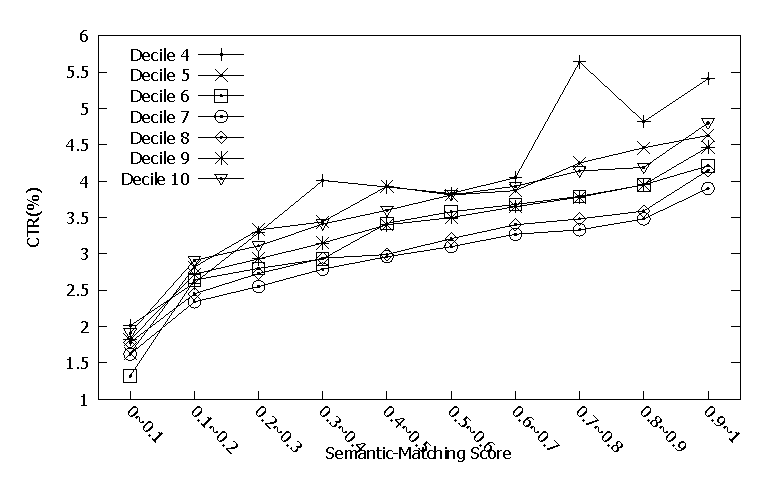
\includegraphics[height=1.2in,
                width=2.2in]{figures/ml.eps}
        \end{minipage}}
    \subfigure[Sidebar Ads] {
        \label{fig*:subfig:f}
        \begin{minipage}[b]{0.33\textwidth}
        \centering
            %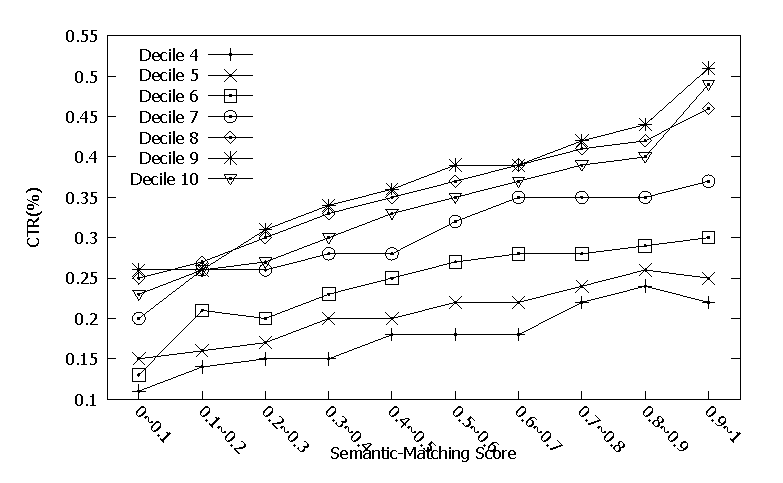
\epsfig{file=figures/sb.eps,height=1.2in,width=2.2in}
            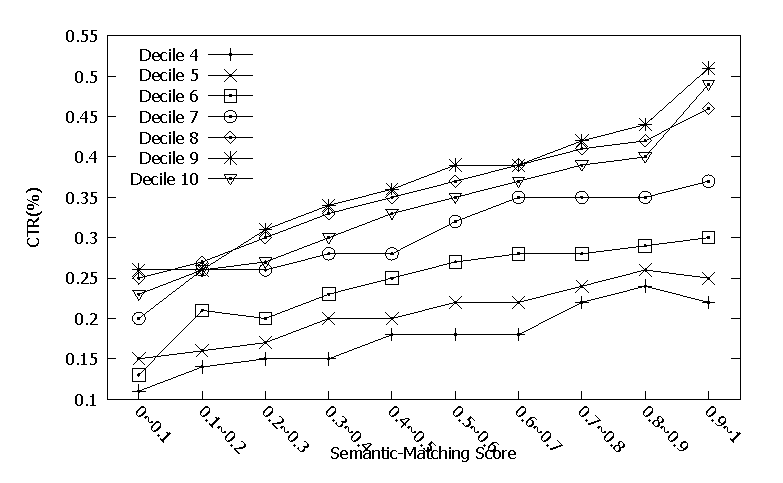
\includegraphics[height=1.2in,
                width=2.2in]{figures/sb.eps}
        \end{minipage}}
    \caption{Correlation between Semantic-Matching Score and CTR}
    \label{fig*:ex1}
\end{figure*}



It is well known that the volume distribution of search queries
follows the power law~\cite{broder:sponsoredsearch}.
We divide the query volume into ten deciles evenly. %in which they have the same total volume of traffic.
\begin{itemize}
\item \emph{Head queries} belong to deciles $1\sim 3$.
They are extremely popular and searched frequently.
\item \emph{Torso queries} belong to deciles $4\sim 6$.
\item \emph{Tail queries} belong to deciles $7\sim 10$.
These queries are rarely accessed and thus have limited historical
data.
\end{itemize}
%Then the frequently accessed queries belong to classes with lower
%decile value while torso and tail queries belong to classes with
%higher decile value.
We show the relationships between SMS and CTR of query-bid phrase pair
for head, torso and tail queries in Figure \ref{fig*:subfig:b},
    \ref{fig*:subfig:c}, \ref{fig*:subfig:d} respectively.
Although SMS fails to reveal the semantic similarity between head
queries and bid phrases accurately, both keyword suggestion and query
expansion for these popular queries have been resolved well.
Consequently, we can leverage co-click signals described in subsection \ref{sec:CSCD} for head queries.
As you can see, for torso and tail queries, there exists a strong
positive correlation between SMS and CTR of query-bid phrase pair, which
confirms the effectiveness of SMS.
Because these queries lack of user behavior data, they can't be covered
by most existing approaches and are research topics of this area.
%By employing semantic knowledge to resolve the bottleneck, our
%approach is helpful for current search engines.



\subsubsection{Ranking by SMS}
\label{sec:smsrank}
\textbf{Objective} of this experiment is to check whether the ranking
determined by SMS is reasonable.
Although the strong correlation between SMS and CTR confirms the effectiveness
of SMS,
%proves that scores assigned
%to bid phrases with regard to a given query are reasonable.
%However, 
    gathering such statistic(i.e., CTR) globally may fail to distinct an
approach that ranks highly relevant bid phrases at the top from
another approach that ranks mildly relevant bid phrases at the top.
%We will take the \emph{order} into consideration in this experiment.
%To show that our approach has the ability to generate reasonable
%ranking for retrieved bid keywords at the top of the result, we
%compare our approach against other mainstream approaches on a dataset
%sampled from search log with Normalized Discounted Cumulated
%Gain(NDCG) as metrics.



\textbf{Dataset} for this experiment are
%search logs accumulated
%during one month period of time by a commercial search engine.
%The search logs consist of about 15.5 billion records within which
%there exist 0.83 billion distinct queries.
%From these search logs, we randomly choose
2504 queries(1000 head
        queries, 1000 torso queries and 504 tail queries) randomly
sampled from our search logs.
Firstly, we computed CTR of query-bid phrase pair for these sampled
queries.
Then we rank each query's bid phrases by their CTRs in descending
order and reserve the top 30 ones (there are only 504 tail queries that
        contain at least 30 bid phrases).
The ranking as well as these bid phrases' CTRs are used as ground
truth for this experiment.



%Since there are a few cases where queries are so relevant to bid
%keywords which are not within their corresponding CTR rank and we don't
%want to revise our dataset manually to avoid loss of objectivity, 
\textbf{Metrics} should take the ranking orders of retrieved bid
phrases into account so that more reasonable rankings can be
distinguished from unreasonable ones.
Thus, we choose Normalized Discounted Cumulated Gain(\emph{NDCG}~\cite{baeza2011modern}) as
    our metrics.
Given a sampled query $q$, aggregate records of search logs to compute
CTR of bid phrases with respect to $q$.
Then we rank bid phrases associates with $q$ by their CTR and reserve
the top 30 bid phrases $(p_{1},\ldots,p_{30})$.
%$(p_{1},\textnormal{CTR}(q,p_1)),\ldots,(p_{30},\textnormal{CTR}(q,p_{30}))$.
We compute the Ideal Discounted Cumulated Gain
(\emph{IDCG}~\cite{baeza2011modern}) of $q$ by
\begin{equation}
\textnormal{IDCG}(q)=\textnormal{CTR}(q,p_1)+\sum_{i=2}^{30}\frac{\textnormal{CTR}(q,p_i)}{\log_{2}i}
\end{equation}
If we rank the top 30 bid phrases of $q$ by some approach, we derive
$p_{f(1)},\ldots,p_{f(30)}$.
Then we compute the Discounted Cumulated Gain (\emph{DCG}~\cite{baeza2011modern}) by
\begin{equation}
\textnormal{DCG}(q)=\textnormal{CTR}(q,p_{f(1)})+\sum_{i=2}^{30}\frac{\textnormal{CTR}(q,p_{f(i)})}{\log_{2}i}
\end{equation}
Finally, NDCG of $q$ can be computed by
\begin{equation}
\textnormal{NDCG}(q)=\frac{\textnormal{DCG}(q)}{\textnormal{IDCG}(q)}
\end{equation}
%The NDCG is defined as %    devided by Ideal Discounted Cumulated Gain(\emph{IDCG}).
%we compute NDCG for each query by ranking the corresponding CTR
%rank of it using CTR value as gain and original CTR rank as ideal
%order to compute Ideal Discounted Cumulated Gain (IDCG).



\textbf{Baselines} include bag-of-words technique,
    pLSA~\cite{hofmann:semanticindexing} and
    ESA~\cite{gabrilovich:semanticanalysis}.
We weight terms using classic TF-IDF scheme and set the number of
topics of pLSA to 100.
TF-IDF weights and probabilities of pLSA model are estimated with
respect to all sampled queries as well as their bid phrases.
%Because bid phrase that has no common terms with its corresponding
%query will not be recalled by bag-of-words technique, we discard such
%kind of bid phrases in re-ranked list.



\begin{figure*}[!ht]
    \subfigure[NDCG on head queries] {
        \label{fig:subfig:a1}
        \begin{minipage}[b]{0.33\textwidth}
            \centering
            %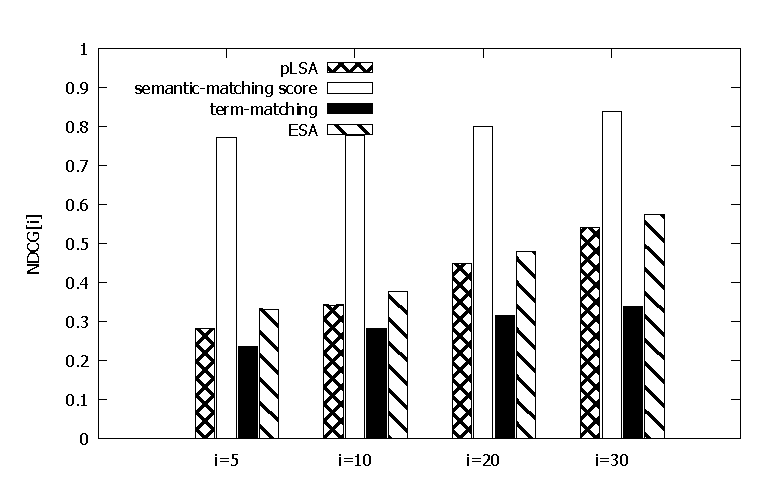
\epsfig{file=figures/headndcg.eps,height=1.2in,width=2.2in}
            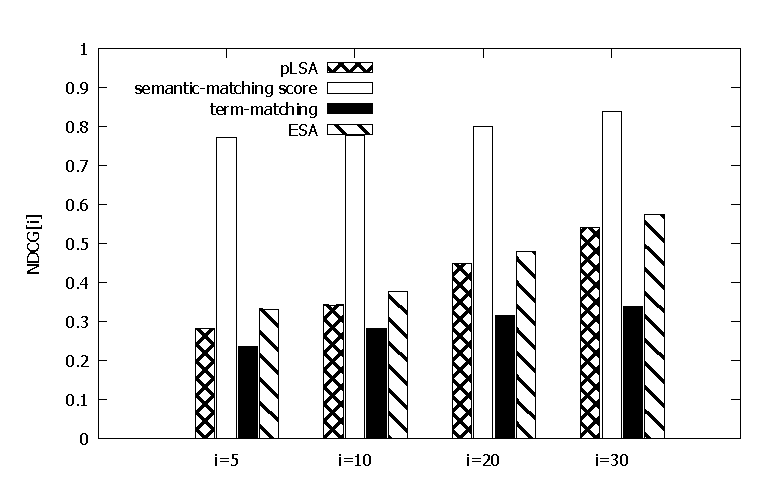
\includegraphics[height=1.2in,
                width=2.2in]{figures/headndcg.eps}
        \end{minipage}
    }
    \subfigure[NDCG on torso queries] {
        \label{fig:subfig:b1}
        \begin{minipage}[b]{0.33\textwidth}
            \centering
            %\epsfig{file=figures/torsondcg.eps,height=1.2in,width=2.2in}
            \includegraphics[height=1.2in,
                width=2.2in]{figures/torsondcg.eps}
        \end{minipage}
    }
    \subfigure[NDCG on tail queries] {
        \label{fig:subfig:c1}
        \begin{minipage}[b]{0.33\textwidth}
            \centering
            %\epsfig{file=figures/tailndcg.eps,height=1.2in,width=2.2in}
            \includegraphics[height=1.2in,
                width=2.2in]{figures/tailndcg.eps}
        \end{minipage}
    }
    \caption{NDCG}
    \label{fig*:ndcg}
\end{figure*}
\textbf{Experiment results} are illustrated in Figure \ref{fig*:ndcg}.
Our approach outperforms baselines under all kinds of settings.
Bag-of-words technique can't recall sufficient bid phrases so it
loses many bid phrases' ``gains'' and results in low NDCG.
Bid phrases' distributions over latent topics are extremely sparse
because each bid phrase contains limited words.
Both ESA and our approach model short texts as explicit concepts and
thus reveal satisfactory coverage and accuracy.
Our approach beats ESA mainly because of the different strategies of
conceptualization.
ESA maps short text into wikipedia's concept space based on
co-occurrence of terms within the short text itself and terms of 
concepts' corresponding articles.
We associate short texts with relevant concepts according to entities
of them.
Since both queries and bid phrases are very short, conceptualization
directly via \emph{isA} relationship is more robust than strategy of
ESA.
\subsection{Retrieval Evaluation}
%Our approach is tasked with selecting relevant bid phrases from a
%massive corpus with respect to a given query.
Approach proposed in this paper intends to match a given query to
relevant bid phrases.
%The resulting bid phrases are retrieved from a extremely huge corpus.
Although previous experiment has confirmed the effectiveness of SMS,
         ranking a small set of bid phrases in a reasonable order is
         only a subproblem of retrieving relevant ones from a
         extremely huge corpus.
Evaluation from the standard IR perspective is indispensable.
\subsubsection{Comparison with Existing Approaches}
\textbf{Dataset} for our evaluation purpose includes a set of testing
queries and a corpus of bid phrases.
We randomly sampled 2554 queries from our search logs as testing
queries.
%sampled from search logs mentioned in Section \ref{sec:smsrank}.
%as our test queries.
%These search logs are accumulated during one month period of time.
%They consist of about 15.5 billion records within
%which there are around 0.83 billion distinct queries.
We also sampled 300,000 bid phrases from our keyword set which have no
common term with our testing queries.
We treat these bid phrases as negative (not relevant) cases if they
appear in the retrieval results of any test query.
Contemporary commercial search engines provide keyword search tools
for advertisers to expand a given query with a list of highly relevant
bid phrases.
%To save labour, we compare our approach with several baselines using
%bid phrases expanded by keyword search tool of a commercial
%search engine.
We make use of keyword search tool provided by a commercial search
engine to expanded our test queries.
%In fact, this keyword search tool fails to provide sufficient number
%of bid phrases for some test queries.
Among the 2554 test queries, 2025 test queries are matched to at least
5 bid phrases and 1845 queries are matched to at least 10 bid phrases.
We regard these bid phrases as positive(relevant) cases if they appear
in the retrieval results of their corresponding test queries.
We merge the 300,000 sampled bid phrases and those provided by tool
together to form our corpus.



\textbf{Metrics} of this experiment includes \emph{p@n} which reflects the relevance between a given query and
its retrieval results, \emph{nonobvious score} which is defined as
one minus the Jaccard Similarity between query and bid phrase where
both the short texts are regarded as set of terms.
In contrast to standard information retrieval which only
focuses on the relevance between query and returned documents, keyword
suggestion also takes the obviousness of keywords into account because
those relevant yet not so obvious bid phrases are not only helpful but
also economical.
For each test query, its \emph{nonobvious score} is defined to be
the average \emph{nonobvious score} of its retrieved bid phrases that
are regared as positive cases.



\textbf{Baselines} includes standard bag of words approach as well as
ESA~\cite{gabrilovich:semanticanalysis}.
To compare our approach with them,
   we apply these approaches to selecting bid phrases for each test
   query from our corpus respectively.
Then we evaluate the retrieval results of different approaches with
our metrics.
%Regarding bid phrases provided by keyword search tool as positive
%cases while others as negative cases, we can compute \emph{p@n
%    (precision at topN)} for
%each query reflecting the relevance between it and its corresponding
%retrieval results.



%We regard each short text as a set of terms and define the
%\emph{nonobvious} of a certain bid phrases and a query as one minus
%the Jaccard Similarity of their corresponding sets of terms.



\textbf{Experiment results} are illustrated in Figure \ref{fig:expadcenter}.
\begin{figure*}[!tb]
    \subfigure[Compare Precision] {
        \label{fig:subfig:a2}
        \begin{minipage}[b]{0.33\textwidth}
            \centering
            %\epsfig{file=figures/precision.eps,height=1.2in,width=2.2in}
            \includegraphics[height=1.2in,
                width=2.2in]{figures/precision.eps}
        \end{minipage}
    }
    \subfigure[Compare Nonobvious]{
        \label{fig:subfig:b2}
        \begin{minipage}[b]{0.33\textwidth}
            \centering
            %\epsfig{file=figures/nonobvious.eps,height=1.2in,width=2.2in}
            \includegraphics[height=1.2in,
                width=2.2in]{figures/nonobvious.eps}
        \end{minipage}
    }
    \subfigure[Compare Precision+Nonobvious]{
        \label{fig:subfig:c2}
        \begin{minipage}[b]{0.33\textwidth}
            \centering
            %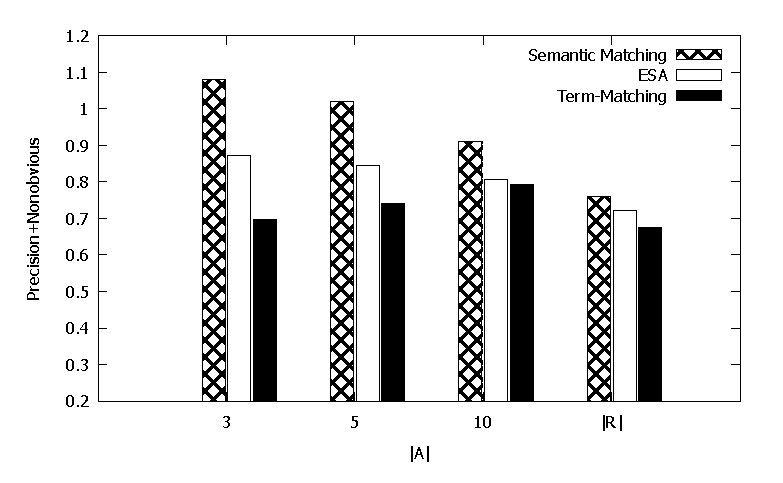
\epsfig{file=figures/plus.eps,height=1.2in,width=2.2in}
            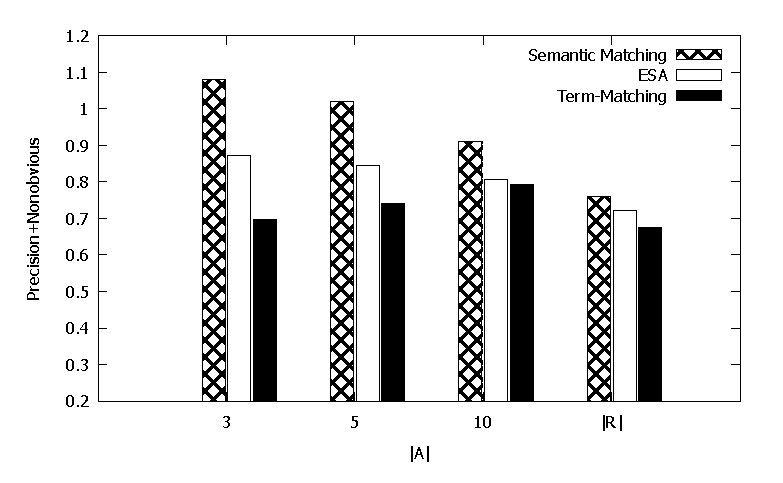
\includegraphics[width=2.2in,
                height=1.2in]{figures/plus.eps}
        \end{minipage}
    }
\caption{Evaluation using Keyword Research Service}
\label{fig:expadcenter}
\end{figure*}
Our semantic matching approach outperform ESA and term-vector
approach on the metrics \emph{p@n} which comfirms the
effectiveness of our approach from the perspective of information
retrieval.
Because both ESA and our approach model short text at semantic
level while standard bag of words technique simply characterizes each
short text as set of terms, the metrics \emph{nonobvious score} is intrinsically
inclined to ESA and our approach.



%\subsubsection{Massive Dataset and User Study}
\subsection{Performance over Massive Dataset}
\textbf{Objective} of this experiment is mainly to confirm the
scalability of our approach.
Besides, since bid phrases provided by keyword search tool is selected
by algorithms instead of human beings, We held user study to assess
the relevance between queries and retrieved bid phrases.



\textbf{Dataset} for our evaluation purpose includes a set of testing
queries and a extremely huge corpus of bid phrases.
For the convenience of user study, we select 50 queries from our query
set that are easy for participators to interpret.
Because previous experiment compare our approach with several
baselines over a corpus of ordinary size(300k bid phrases), we
adopt the whole keyword set for this experiment.



\textbf{Metrics} of this experiment is p@n.
Because our human resource is limited, we give up graded relevance
assessments such as NDCG and thus choose p@n which allow only binary
assessments.
For each test query, we apply different approaches to selecting bid
phrases from our massive corpus respectively.
Then participators are asked to label each result as relevant or not
according to their own subjective judgment.
There are totally five participators and all of them are experienced
web users.



%For each of these sampled queries, we select top-$10$ bid phrases by our
%approach from a huge corpus consisting of 0.702 billion bid phrases
%provided by a commercial search engine.
%We adopt such a extremely huge corpus to confirm that our approach has
%the scalability to be applied for such massive dataset.
%These queries' most relevant expansions are also extracted to be used
%as baseline\comment{what?}.
\textbf{Baseline} of this experiment is not certain keyword suggestion
or query expansion approach.
%, but the most successful bid phrases with
%respect to our test queries provided by a commercial search engine.
Instead, we use each test query's expansions provided by commercial
search engine as baseline.
The expansions of queries are bid phrases which have the highest
\emph{CTR}.
%Participators are asked to score each resulting bid phrase according to labeling guidline listed in Table
%\ref{tab:scoringrule} without the information that bid
%phrases are generated by a certain approach.

%Since our corpus consists of totally 0.702 billion bid phrases, it's impossible
%for human beings to count the exact number of relevant ones with
%respect to a given query within the corpus.
%Thus, we compared the quality of expansions generated by our
%approach and those provided by search engine using \emph{p@n} as
%metrics.
%Because we asked users to label results in a stage manner(i.e., we do
%        not label bid phrases as black or white but assign a score to
%        each one), we define \emph{p@n} slightly different from
%conventional one.
%Actually, we define it to be the summation of labeled scores of top-$n$
%bid phrases divided by $3\times n$.
%We consider cases where $n=1, 3, 5, 10$.
%The comparison is illustrated in the Table \ref{tab:vsbing}.
For some test queries, the number of relevant bid phrases provided by
the search engine is less than 10, so we have to present the
\emph{p@10} only of our approach.



\textbf{Experiment results} are illustrated in Table \ref{tab:vsbing}.
For small $n$, our approach achieve obvious
improvement compared with the commercial search engine.
Because the number of ads displayed for one search is much less
than the number of web pages returned to search users, the relevance
between top ranked bid phrases and given query is critical.
Therefore, the advantage of our approach is significant.
%We have claimed that our approach is suitable for applying to massive
%dataset, so we evaluate our approach using 702 millions of bid
%keywords indexed by Bing search engine.
%We randomly sampled 42 quries including head queries as well as torso
%and tail queries, from search log and generate top 5 most related bid
%keywords for each query as resulting expansion by our approach.
%We also extracted the expansion results for these queries generated by
%Bing search engine.
%For comparison purpose, we held user study where each participator is
%asked to score each resulting bid keyword according to pre-defined
%rule.
%Table \ref{tab:scoringrule} presents scoring rule adopted in our user study.
%We labeled resulting bid keywords in a stage manner expecting to give
%them more precise description and present the relationship between
%queries and bid keywords rather than simply judging them as relevant
%or not.
%\begin{table}
%\centering
%\caption{Scoring Rule}
%\begin{tabular}{|c|c|c|c|} \hline
%Score&Relationship&Query&Bid Keyword\\ \hline
%3&same&car insurance&automatic insurance\\ \hline
%2&specific&car rental&car rental LA\\ \hline
%2&general&iphone&apple product\\ \hline
%2&overlap&fruit ninja xbox&fruit ninja for ios\\ \hline
%1&disjoint&hot dog&dog\\ \hline
%\end{tabular}
%\label{tab:scoringrule}
%\end{table}
%Since the total corpus contains about 702 millions of bid keywords, we
%have no idea about the exact number of related bid keywords for a given
%query which is required for computing precision and recall.
%We compared the performance of our approach with Bing search engine by
%comparing \emph{p@n} which is also a conventional metrics for evaluating
%informaion retrieval systems.
%Here we consider cases where $n=1, 3, 5$.
%As we know, \emph{p@n} is computed by dividing the number of positive
%ones in the top-$n$ by $n$ where testing data is labeled in a black or
%white manner.
%So we have to make some modification to \emph{p@n} for our cases.
%Here we define it to be the summation of scores of top-$n$ bid
%keywords divided by $3\times n$.
%The comparison is illustrated in the Table 3.
\begin{table}
\centering
\begin{tabular}{|c|c|c|} \hline
$p@n$&Search Engine&Our Approach\\ \hline
$n=1$&$0.778$&$0.827$\\ \hline
$n=3$&$0.729$&$0.784$\\ \hline
$n=5$&$0.723$&$0.755$\\ \hline
$n=10$&&$0.717$\\ \hline
\end{tabular}
\caption{Comparison between Our Approach and Bing Search Engine}
\label{tab:vsbing}
\end{table}
%\subsection{Pruning}
%In reality, search engine preprocesses a list of queries offline and
%builds inverted index for the resulting expansions(query as term and
%    its expansion as corresponding posting list).
%At runtime, search engine uses the resulting expansions to find
%relevant bid keywords for submitted query.
%When there is enough traffic volumne to ensure computed metrics(e.g.,
%        click through rate(CTR), cost per click(CPC), etc.) reliable,
%     search engine will analyze and prune those bad expansion.
%For example, a certain bid keyword is high-ranking in the expansion
%for a certain query.
%However, the CTR for ads retrieved through this bid keyword is so low.
%This bid keyword may be not so relevant to that query and search
%engine will eliminate it from that query's expansion in the next
%version.
%Although pruning is not an elegant approach to improve effectiveness
%of sponsored search, it is an important and indespensable step of
%sponsored search adopted by many mainstream search engines.
%
%
%Different from latent semantic analysis approaches which represent
%documents as distribution over latent topics and topics as
%distributions over vocabulary of indexed corpus, our approach
%represents documents as explicit topics where topics are concepts used
%in our daily life.
%Such a representation of the meaning behind any text is
%easy to explain to human users\cite{gabrilovich:semanticanalysis}.
%By our explicit representation of semantic meaning, we are able to not
%only prune resulting expansion based on conventioinal metrics but also
%infer and analyze more detailed problem behind the symptom such as
%which topics(concepts) contain commercial intent, which domains our
%approach can't not generate useful expansions.
%For example, when we find that CTRs of expansions for queries related
%to concept ``hotel'' are lower than other topics(concepts),
%we can collect these queries and design vertical search engine for
%this specific domain.
